%%% Copyright (C) 2017 Vincent Goulet
%%%
%%% This file and all files included or input by this one (and
%%% recursively) are part of the project "Computational actuarial
%%% science with R - IME 2017 Workshop"
%%% http://github.com/vigou3/ime-2017-workshop-computational-actuarial-science-r
%%%
%%% This work is licensed under a Creative Commons
%%% Attribution-ShareAlike 4.0 International License.
%%% http://creativecommons.org/licenses/by-sa/4.0/

\documentclass[aspectratio=1610,10pt,xcolor=x11names]{beamer}
  \usepackage[noae]{Sweave}
  \usepackage[round]{natbib}             % references
  \usepackage{fontawesome}               % various icons
  \usepackage{awesomebox}                % tipbox et al.
  \usepackage{changepage}                % license page
  \usepackage{listings}                  % source code
  \usepackage{tabularx}                  % license page
  \usepackage{framed}                    % env. leftbar
  \usepackage[export]{adjustbox}         % frame around image
  \usepackage[overlay,absolute]{textpos} % covers
  \usepackage{metalogo}                  % logo \XeLaTeX
  \usepackage{bm}                        % bold math for vectors

  %% ==================
  %%  Publication info
  %% ==================
  \renewcommand{\year}{2017}

  %% ===============================
  %%  Look and feel of the document
  %% ===============================

  %% Beamer theme
  \usetheme{metropolis}

  %% Math in sans serif font
  \usepackage[frenchmath,nosymbolsc,scaled=1.15]{newtxsf}

  %% Additionnal colors
  \definecolor{comments}{rgb}{0.7,0,0}      % comments in R code
  \definecolor{link}{rgb}{0,0.4,0.6}        % internal links
  \definecolor{url}{rgb}{0.6,0,0}           % external links
  \definecolor{codebg}{named}{LightYellow1} % R code background
  \definecolor{rouge}{rgb}{0.85,0,0.07}     % UL red stripe
  \definecolor{or}{rgb}{1,0.8,0}            % UL yellow stripe
  \colorlet{alert}{mLightBrown} % alias for Metropolis color
  \colorlet{dark}{mDarkTeal}    % alias for Metropolis color
  \colorlet{shadecolor}{codebg}

  %% Hyperlinks
  \hypersetup{%
    pdfauthor = {Vincent Goulet},
    pdftitle = {Computational actuarial science with R},
    colorlinks = {true},
    linktocpage = {true},
    allcolors = {link},
    urlcolor = {url},
    pdfpagemode = {UseOutlines},
    pdfstartview = {Fit},
    bookmarksopen = {true},
    bookmarksnumbered = {true},
    bookmarksdepth = {subsection}}

  %% Source code blocks
  \lstloadlanguages{R}
  \lstset{language=R,
    extendedchars=true,
    basicstyle=\small\ttfamily,
    commentstyle=\color{comments}\slshape,
    keywordstyle=\mdseries,
    escapeinside=`',
    aboveskip=0pt,
    belowskip=0pt,
    showstringspaces=false}

  %% Bibliography
  %% Couple of hacks needed to have beamer and natbib play nice with
  %% each other.
  \renewcommand{\newblock}{}    % https://tex.stackexchange.com/a/1971/24355
  \renewcommand{\bibsection}{}  % drop \section heading
  \bibliographystyle{abbrvnat}

  %% ===============================
  %%  New commands and environments
  %% ===============================

  %% Sweave environments Sinput and Soutput use Verbatim (from
  %% fancyvrb). They are redefined to remove the default configuration
  %% of Sweave and we reduce spacing between the Sinput and Soutput
  %% blocks.
  \DefineVerbatimEnvironment{Sinput}{Verbatim}{}
  \DefineVerbatimEnvironment{Soutput}{Verbatim}{}
  \fvset{fontsize=\small,listparameters={\setlength{\topsep}{0pt}}}

  %% Environment Schunk completely redefined as an hybrid between
  %% environments snugshade* and leftbar of framed.
  \makeatletter
  \renewenvironment{Schunk}{%
    \def\FrameCommand##1{\hskip\@totalleftmargin
      \vrule width 3pt\colorbox{codebg}{\hspace{5pt}##1}%
      % There is no \@totalrightmargin, so:
      \hskip-\linewidth \hskip-\@totalleftmargin \hskip\columnwidth}%
    \MakeFramed {\advance\hsize-\width
      \@totalleftmargin\z@ \linewidth\hsize
      \advance\labelsep\fboxsep
      \@setminipage}%
  }{\par\unskip\@minipagefalse\endMakeFramed}
  \makeatother

  %% Theorem-like environments
  \theoremstyle{plain}
  \newtheorem{assumption}{Assumption}
  \theoremstyle{definition}
  \newtheorem{consequence}{Consequence}

  %% Function names, code, arguments et al.
  \newcommand{\code}[1]{\texttt{#1}}
  \newcommand{\file}[1]{\fbox{\code{#1}}}
  \newcommand{\class}[1]{\textbf{#1}}
  \newcommand{\pkg}[1]{\textbf{#1}}
  \newcommand{\link}[2]{\href{#1}{#2~\raisebox{-0.2ex}{\faExternalLink}}}
  \newcommand{\meta}[1]{\ensuremath\langle{\normalfont\itshape #1\/}\ensuremath\rangle}

  %% Link to GitHub on copyright page
  \newcommand{\viewsource}[1]{%
    \href{#1}{%
      View on GitHub \raisebox{-1pt}{\footnotesize\faGithub}}}

  %% Link to R scripts
  \newcommand{\gotoR}[1]{%
    \begin{center}
      \colorbox{dark}{\color{white}
      \makebox[40mm][c]{%
        \makebox[5mm]{\raisebox{-1pt}{\large\faChevronCircleDown}}\;%
        {\ttfamily #1}}}
    \end{center}}

  %% Context-specific commands
  \newcommand{\mat}[1]{\bm{#1}}
  \newcommand{\esp}[1]{E [ #1 ]}
  \newcommand{\VaR}{\ensuremath{\text{VaR}}}
  \newcommand{\TVaR}{\ensuremath{\text{TVaR}}}
  \newcommand{\feu}{{[\text{F}]}}
  \newcommand{\eau}{{[\text{W}]}}
  \newcommand{\bris}{{[\text{A}]}}
  \newcommand{\DOT}{{[\ast]}}

  %%% =======
  %%%  Varia
  %%% =======

  %% Lengths to compose front and rear covers.
  \newlength{\banderougewidth} \newlength{\banderougeheight}
  \newlength{\bandeorwidth}    \newlength{\bandeorheight}
  \newlength{\imageheight}     \newlength{\imagewidth}
  \newlength{\logoheight}
  \newlength{\gapwidth}

%  \includeonly{licence}

\begin{document}

%% frontmatter
\begingroup

\TPGrid{3}{36}
\textblockorigin{0mm}{0mm}
\setlength{\parindent}{0mm}
\setlength{\banderougewidth}{2\TPHorizModule}
\setlength{\banderougeheight}{\TPVertModule}
\setlength{\bandeorwidth}{\TPHorizModule}
\setlength{\bandeorheight}{\banderougeheight}
\setlength{\imageheight}{29\TPVertModule}
\setlength{\imagewidth}{3\TPHorizModule}
\setlength{\logoheight}{2.5\TPVertModule}
\setlength{\gapwidth}{0.75pt}
\addtolength{\bandeorwidth}{-\gapwidth}
\addtolength{\imageheight}{-\gapwidth}

\begin{frame}[plain]
  %% UL banner
  \begin{textblock*}{3\TPHorizModule}[0,1](0mm,30\TPVertModule)
    \textcolor{rouge}{\rule{\banderougewidth}{\banderougeheight}}% % red stripe
    \rule{\gapwidth}{0pt}%                                         % gap
    \textcolor{or}{\rule{\bandeorwidth}{\bandeorheight}}           % gold stripe
  \end{textblock*}

  %% UL logo
  \begin{textblock*}{\TPHorizModule}(2\TPHorizModule,31\TPVertModule)
    \rule{\gapwidth}{0pt}%                                     % gap
    \includegraphics[height=\logoheight,keepaspectratio=true]{ul_p}
  \end{textblock*}

  %% background image
  \begin{textblock*}{3\TPHorizModule}(0mm,0mm)
    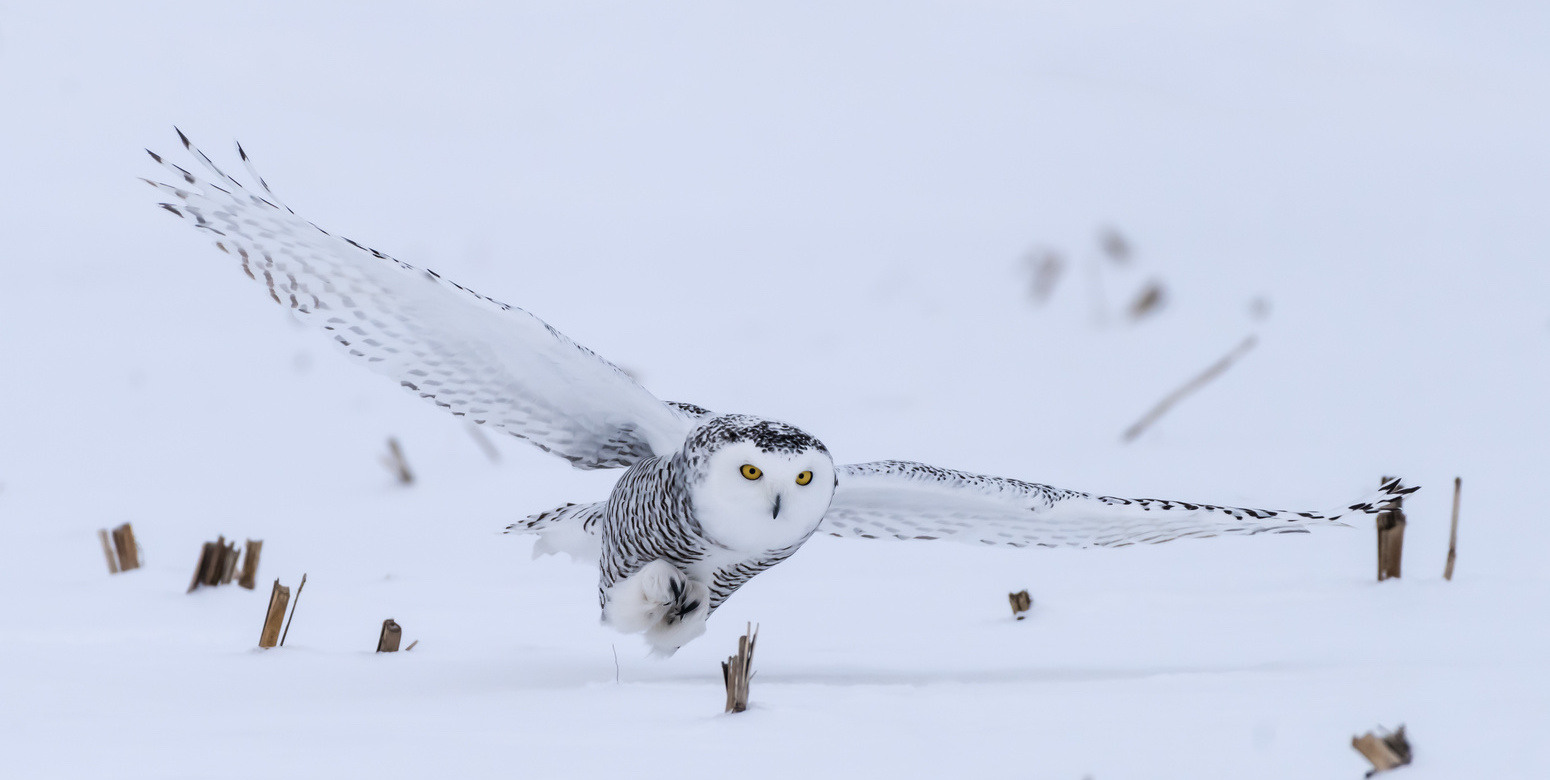
\includegraphics[height=\imageheight,width=\imagewidth]{Fotolia_99831160.jpg}
    %\includegraphics[height=\imageheight,width=\imagewidth]{Klimt.jpg}
    %\includegraphics[height=\imageheight,width=\imagewidth]{Eulen_an_Fassade_TU_Bibliothek}
  \end{textblock*}

  %% title
  \begin{textblock*}{2.6\TPHorizModule}(0.2\TPHorizModule,3\TPVertModule)
    \raggedright%
    \bfseries
    \fontsize{22}{22}\selectfont
    Computational actuarial science with R \\
    \mdseries
    \fontsize{12}{13}\selectfont
    Workshop of the 21\textsuperscript{st} International Congress on
    Insurance: \\ Mathematics and Economics -- IME 2017
  \end{textblock*}

  %% date
  \begin{textblock*}{2\TPHorizModule}(0.2\TPHorizModule,26\TPVertModule)
    \fontsize{10}{12}\selectfont
    July 6-7, 2017
  \end{textblock*}
\end{frame}
\endgroup

%%% Local Variables:
%%% mode: latex
%%% TeX-engine: xetex
%%% TeX-master: "ime-2017-workshop-computational-actuarial-science-r"
%%% End:

\begingroup

\TPGrid{3}{36}
\textblockorigin{0mm}{0mm}
\begin{frame}[plain]
  %% title
  \begin{textblock*}{2.6\TPHorizModule}(0.2\TPHorizModule,3\TPVertModule)
    \raggedright%
    \bfseries
    \fontsize{22}{22}\selectfont
    Computational actuarial science with R \\
    \mdseries
    \fontsize{12}{13}\selectfont
    Workshop of the 21\textsuperscript{st} International Congress on
    Insurance: \\ Mathematics and Economics -- IME 2017
  \end{textblock*}

  %% author
  \begin{textblock*}{2\TPHorizModule}(0.2\TPHorizModule,15\TPVertModule)
    \fontsize{10}{11}\selectfont
    \bfseries
    Vincent Goulet \\
    \fontsize{9}{11}\selectfont
    \mdseries
    Full Professor | École d'actuariat, Université Laval
  \end{textblock*}
\end{frame}
\endgroup

%%% Local Variables:
%%% mode: latex
%%% TeX-engine: xetex
%%% TeX-master: "ime-2017-workshop-computational-actuarial-science-r"
%%% End:

%%% Texte du contrat de licence au début des diapos

\begin{frame}[t,plain,fragile=singleslide]
  \tiny
  \vspace*{10mm}

  \begin{adjustwidth}{15mm}{15mm}
    {\textcopyright} {\year} Vincent Goulet \\[4mm]

    
\includegraphics[height=4mm,keepaspectratio=true]{by-sa} \\%

    This work is licensed under a Creative Commons
    \href{http://creativecommons.org/licenses/by-sa/4.0/deed.en}{%
      Attribution-ShareAlike 4.0 International}
    license. You are free to:
    \begin{itemize}
    \item \textbf{Share} --- copy and redistribute the material in any
      medium or format;
    \item \textbf{Adapt} --- remix, transform, and build upon the
      material for any purpose, even commercially.
    \end{itemize}
    Under the following terms: \vspace*{2mm}

    \begin{tabularx}{\linewidth}{@{}lX@{}}
      \raisebox{-5.5mm}[0mm][7mm]{%
        
\includegraphics[height=7mm,keepaspectratio=true]{by}} &
      \textbf{Attribution} --- You must give appropriate credit,
      provide a link to the license, and indicate if changes were
      made. You may do so in any reasonable manner, but not in any way
      that suggests the licensor endorses you or your use. \\
      \raisebox{-5.5mm}{
\includegraphics[height=7mm,keepaspectratio=true]{sa}}
      & \textbf{ShareAlike} --- If you remix, transform, or build upon
      the material, you must distribute your contributions under the
      same license as the original. \\
      & \textbf{No additional restrictions} --— You may not apply
      legal terms or technological measures that legally restrict
      others from doing anything the license permits.
    \end{tabularx}
    \vspace{2mm}

    \textbf{Source code} \\
    \viewsource{https://github.com/vigou3/ime-2017-workshop-computational-actuarial-science-r/}
    \vspace{2mm}

    \textbf{Cover} \\
    The bird on the cover is a snowy owl (\emph{Nyctea scandiaca}).
    The National Assembly of Québec adopted the snowy owl as official
    bird in 1987 as a symbol of the province’s support for wildlife
    protection.
  \end{adjustwidth}
\end{frame}

%%% Local Variables:
%%% mode: latex
%%% TeX-engine: xetex
%%% TeX-master: "ime-2017-workshop-computational-actuarial-science-r"
%%% End:


%% mainmatter
\part{R programming}
\frame{\partpage}

\include{presentation}
\include{fundamentals}
\include{datatypes}
\section{Mapping functions}

\begin{frame}[fragile]
  \frametitle{The  \code{apply} family of functions}

  Efficient tools for data reduction and repeated computations.

  \begin{itemize}
  \item \code{apply} applies a function to margins of a \alert{matrix}
    or \alert{array}.
    \begin{Schunk}
\begin{lstlisting}
apply(X, MARGIN, FUN, ...)
\end{lstlisting}
    \end{Schunk}

  \item \code{tapply} applies a function to each \alert{group of
      values} given by categories of \alert{factors}.
    \begin{Schunk}
\begin{lstlisting}
tapply(X, INDEX, FUN, ...)
\end{lstlisting}
    \end{Schunk}
    Similar and sometimes easier to use: \code{by}, \code{aggregate}.

  \item \code{lapply} and \code{sapply} apply a function to each
    element of a \alert{vector} or \alert{list}.
    \begin{Schunk}
\begin{lstlisting}
lapply(X, FUN, ...)
sapply(X, FUN, ...)
\end{lstlisting}
    \end{Schunk}
    Also in the same family: \code{mapply}.
  \end{itemize}
  \pause
  \gotoR{application.R}
\end{frame}

%%% Local Variables:
%%% mode: latex
%%% TeX-engine: xetex
%%% TeX-master: "ime-2017-workshop-computational-actuarial-science-r"
%%% End:

\section{Control structures}

\begin{frame}[fragile=singleslide]
  \frametitle{Conditional execution}

  \begin{minipage}{\linewidth}
    \begin{minipage}[t]{0.48\linewidth}
      \begin{Schunk}
\begin{lstlisting}
if (`\meta{condition}')
    `\meta{consequence}'
\end{lstlisting}
      \end{Schunk}
    \end{minipage}
    \hfill
    \begin{minipage}[t]{0.48\linewidth}
      \begin{Schunk}
\begin{lstlisting}
if (`\meta{condition}')
    `\meta{consequence}'
else
    `\meta{alternative}'
\end{lstlisting}
      \end{Schunk}
    \end{minipage} \\
    \mbox{}
  \end{minipage}
  \begin{itemize}
  \item \meta{condition} statement evaluating to \alert{unique} value
    \texttt{TRUE} or \texttt{FALSE}
    \begin{itemize}
    \item useful: \verb=all=, \verb=any=,
      \verb=isTRUE=, \dots
    \item useless: \verb|if (TRUE == TRUE)|
    \end{itemize}
  \item \meta{consequence} statement, or group of statements, to execute
    when condition is \texttt{TRUE}
  \item \meta{alternative} statement, or group of statements, to execute
    when condition is \texttt{FALSE}
  \end{itemize}
\end{frame}

\begin{frame}
  \frametitle{Repeated execution}

  \tipbox{
    \begin{itemize}
    \item First try to vectorize calculations
    \item Use functions
      \begin{itemize}
      \item \texttt{outer}
      \item \texttt{apply}
      \item \texttt{tapply}
      \item \texttt{lapply}, \texttt{sapply}
      \item \texttt{mapply}
      \end{itemize}
    \end{itemize}}
\end{frame}

\begin{frame}[fragile=singleslide]
  \frametitle{Three types of loops}

  Number of repetitions known.
  \begin{Schunk}
\begin{lstlisting}
for (`\meta{variable}' in `\meta{sequence}')
    `\meta{statement}'
\end{lstlisting}
  \end{Schunk}

  Number of repetitions unknown, maybe never executed.
  \begin{Schunk}
\begin{lstlisting}
while (`\meta{condition}')
    `\meta{statement}'
\end{lstlisting}
  \end{Schunk}

  Number of repetitions unknown, executed at least once.
  \begin{Schunk}
\begin{lstlisting}
repeat
    `\meta{statement}'
\end{lstlisting}
  \end{Schunk}
\end{frame}

\begin{frame}
  \frametitle{Flow control}

  \begin{itemize}
  \item \texttt{break} causes exit from innermost loop
  \item \texttt{next} forces execution of the next iteration of
    the loop
  \item \texttt{stop()} forces exit from function with error message
  \item \texttt{warning()} forces exit from function with warning
  \item \texttt{return()} forces exit from function with value
  \end{itemize}

  \pause
  \gotoR{control.R}
\end{frame}

%%% Local Variables:
%%% mode: latex
%%% TeX-engine: xetex
%%% TeX-master: "ime-2017-workshop-computational-actuarial-science-r"
%%% End:

\section{Extensions}

\begin{frame}[fragile=singleslide]
  \frametitle{Library and packages}

  \begin{itemize}
  \item Functions, data and documentation distributed as \alert{packages}
  \item Packages collected into \alert{libraries}
  \item Standard library of R contains 29 packages, some of which
    loaded by default at start-up
  \item Load package in memory with
    \begin{Schunk}
\begin{lstlisting}
library(`\meta{package}')
\end{lstlisting}
    \end{Schunk}
  \item Install new package from
    \link{https://cran.r-project.org}{CRAN} with
    \begin{Schunk}
\begin{lstlisting}
install.packages(`\meta{package}')
\end{lstlisting}
    \end{Schunk}
  \end{itemize}
\end{frame}

\begin{frame}[fragile=singleslide]
  \frametitle{Personal library}

  I highly recommend settin up a personal library for extension
  packages.

  \begin{enumerate}
  \item Identify your \verb=~= (\alert{home}) directory with, from R
    \begin{Schunk}
\begin{lstlisting}
> Sys.getenv("HOME")
\end{lstlisting}
    \end{Schunk}
  \item Create a directory within \verb=~=, e.g.
    \begin{Schunk}
\begin{lstlisting}
~/R/library
\end{lstlisting}
    \end{Schunk}
  \item Specify the location of the library in file
    \verb=~/.Renviron= with a line of the form
    \begin{Schunk}
\begin{lstlisting}
R_LIBS_USER="~/R/library"
\end{lstlisting}
    \end{Schunk}
  \end{enumerate}

  \pause
  \gotoR{extensions.R}
\end{frame}

%%% Local Variables:
%%% mode: latex
%%% TeX-engine: xetex
%%% TeX-master: "ime-2017-workshop-computational-actuarial-science-r"
%%% End:

\include{floatingpoint}
\include{speed}

\part{Case study}
\frame{\partpage}

\section{Pricing of individual objects}

\begin{frame}
  \frametitle{Inspiration}

  \begin{center}
    
\includegraphics[width=0.8\linewidth,keepaspectratio,frame]{ime-2017-insurance-of-things} \\
    \link{https://github.com/vigou3/ime-2017-insurance-of-things/releases/tag/v1.0}{Slides
      available on GitHub}
  \end{center}
\end{frame}

\begin{frame}
  \frametitle{Different types of peril}

  \begin{assumption}
    Claims due to three main types of peril:
    \begin{enumerate}
    \item accidental damage, theft, vandalism; \alert{few} items affected ($<$ 10 on average)
    \item fire; \alert{100\%} of items affected
    \item flooding, water damage, sewer backup; \alert{25\%} of items
      affected
    \end{enumerate}
  \end{assumption}
  \pause

  \begin{consequence}
    Aggregate claim amount for insured $i = 1, \dots, n$ for one period:
    \begin{equation*}
      S_i = S_i^\bris + S_i^\feu + S_i^\eau
    \end{equation*}
  \end{consequence}
\end{frame}

\begin{frame}
  \frametitle{Dependence -- Step I}

  \begin{assumption}
    Aggregate claim amount for a given type of peril is compound Poisson:
    \begin{equation*}
      S_i^\DOT = X_{i1}^\DOT + \dots + X_{iN_i^\DOT}^\DOT
      \sim \text{Compound Poisson}(\lambda^\DOT, F^\DOT)
    \end{equation*}
  \end{assumption}
  \pause

  \begin{consequence}
    Aggregate claim amount for insured $i$ is compound Poisson:
    \begin{equation*}
      S_i = S_i^\bris + S_i^\feu + S_i^\eau \sim
      \text{Compound Poisson}(\lambda, F),
    \end{equation*}
    with
    \begin{align*}
      \lambda &= \lambda^\bris + \lambda^\feu + \lambda^\eau \\
      F(x) &= \frac{\lambda^\bris F^\bris(x) + \lambda^\feu F^\feu(x) +
               \lambda^\eau F^\eau(x)}{\lambda}
      \end{align*}
  \end{consequence}
\end{frame}

\begin{frame}
  \frametitle{Dependence -- Step II}

  \begin{assumption}
    Amount of single claim is
    \begin{equation*}
      X_{ij}^\DOT = V_1 + ... + V_{M_{ij}^\DOT},
    \end{equation*}
    where
    \begin{itemize}
    \item $M^\DOT$ is the number of items affected (strictly
      positive discrete distribution)
    \item $V$ is the value of an item (i.i.d.)
    \end{itemize}
  \end{assumption}
  \pause

  \begin{consequence}
    $X_{ij}^\DOT$ is a compound zero-truncated
  \end{consequence}
\end{frame}

\begin{frame}
  \frametitle{Parametrization}

  We need to determine the following elements from judgment, expert
  opinion or collateral data:
  \begin{itemize}
  \item Poisson parameters $\lambda^\bris$, $\lambda^\feu$ and
    $\lambda^\eau$ for the number of claims by type of peril
  \item Zero-truncated distributions of the number of items affected
    per type of peril
  \item Market value of an item
  \end{itemize}
\end{frame}

\begin{frame}
  \frametitle{Pricing}

  \begin{itemize}
  \item Average aggregate claim amount in portfolio:
    \begin{equation*}
      W = \frac{S_1 + \dots + S_n}{n}
    \end{equation*}
  \item<2-> Pure premium: $\esp{W}$
  \item<3-> Premium with safety loading:
    \begin{equation*}
      \pi = \TVaR_\alpha(W) = \esp{W|W > \VaR_\alpha(W)}
    \end{equation*}
  \end{itemize}
\end{frame}


%%% Local Variables:
%%% mode: latex
%%% TeX-engine: xetex
%%% TeX-master: "ime-2017-workshop-computational-actuarial-science-r"
%%% End:

\section{Literate programming}

\begin{frame}
  \frametitle{Increase your productivity}

  You want to use literate programming with R.
  \begin{itemize}
  \item Concept: documentation and source code woven together in a
    file
  \item {\LaTeX} users:
    \link{https://stat.ethz.ch/R-manual/R-devel/library/utils/doc/Sweave.pdf}{Sweave}
  \item Non (yet!) {\LaTeX} users:
    \link{http://rmarkdown.rstudio.com}{Rmarkdown}
  \end{itemize}
\end{frame}

%%% Local Variables:
%%% mode: latex
%%% TeX-engine: xetex
%%% TeX-master: "ime-2017-workshop-computational-actuarial-science-r"
%%% End:


%% backmatter
\begin{frame}[allowframebreaks]
  \frametitle{References}

  \bibliography{stat,vg,informatique,r}
\end{frame}

%%% Local Variables:
%%% mode: latex
%%% TeX-engine: xetex
%%% TeX-master: "ime-2017-workshop-computational-actuarial-science-r"
%%% End:

\begin{frame}[plain]
  \begin{adjustwidth}{20mm}{20mm}
    \scriptsize \raggedright %
    This document was typeset with {\XeLaTeX} using the
    \textbf{beamer} class and the Metropolis theme. Text is in Fira
    Sans, code is in Fira Mono, mathematics are in STIX Math
    Sans-serif and icons come from Font~Awesome.
  \end{adjustwidth}
\end{frame}

%%% Local Variables:
%%% mode: latex
%%% TeX-engine: xetex
%%% TeX-master: "ime-2017-workshop-computational-actuarial-science-r"
%%% End:

\begingroup

\TPGrid{3}{36}
\textblockorigin{0mm}{0mm}
\setlength{\parindent}{0mm}
\setlength{\banderougewidth}{2\TPHorizModule}
\setlength{\bandeorwidth}{\TPHorizModule}
\setlength{\gapwidth}{0.75pt}
\addtolength{\bandeorwidth}{-\gapwidth}

\begin{frame}[plain]
  \begin{textblock*}{125mm}[0,1](0mm,30\TPVertModule)
    \textcolor{or}{\rule{\bandeorwidth}{\TPVertModule}}%      % gold stripe
    \rule{\gapwidth}{0pt}%                                    % gap
    \textcolor{rouge}{\rule{\banderougewidth}{\TPVertModule}} % red stripe
  \end{textblock*}
\end{frame}
\endgroup

%%% Local Variables:
%%% mode: latex
%%% TeX-engine: xetex
%%% TeX-master: "ime-2017-workshop-computational-actuarial-science-r"
%%% End:


\end{document}

%%% Local Variables:
%%% mode: latex
%%% TeX-engine: xetex
%%% TeX-master: t
%%% End:
